%<dscrpt>Autour des polynômes d'interpolation et d'un lemme de Stieltjes.</dscrpt>
Si $P$ est un polynôme à coefficients réels et $x$ un nombre réel, on convient de noter $\widetilde{P}(x)$ le nombre réel obtenu en substituant $x$ à X dans $P$.\newline
Dans tout le problème, $n$ et $k$ sont deux entiers fixés:
\begin{align*}
 n\geq 3 & & 1<k<n
\end{align*}
Pour tout entier $m$, $\R_{m}[X]$ désigne le $\R$-espace vectoriel formé par les polynômes de degré inférieur ou égal à $m$ et le polynôme nul. On note en particulier 
\begin{align*}
 E = \R_{2n-2}[X] & & A = \R_{n-1}[X]
\end{align*}
On se donne $n$ nombres réels 
\begin{displaymath}
 x_1 < x_2 < \cdots < x_n
\end{displaymath}
Il est à noter que, parmi ces nombres, $x_k$ (avec $k$ fixé au début) va jouer un rôle particulier.
On définit le polynôme $L$ :
\begin{displaymath}
 L = (X-x_1)(X-x_2)\cdots (X-x_n)
\end{displaymath}
Pour chaque entier $i$ entre $1$ et $n$, on définit un polynôme $L_i$  par :
\begin{displaymath}
L_i = \prod_{j\in\{1,\cdots,n\}-\{i\}}\frac{X-x_j}{x_i-x_j} 
\end{displaymath}

\subsection*{Partie I}
On définit une application $\Phi$  de $E$ dans $\R^{2n-1}$ par :
\begin{displaymath}
 P \rightarrow \left( \widetilde{P}(x_1),\widetilde{P}(x_2),\cdots,\widetilde{P}(x_n),
 \widetilde{P'}(x_1),\cdots ,\widetilde{P'}(x_{k-1}),\widetilde{P'}(x_{k+1}),\cdots,\widetilde{P'}(x_n)\right) 
\end{displaymath}
Il est à noter que $\widetilde{P'}(x_{k})$ \emph{ne figure pas} dans la famille.
\begin{enumerate}
\item Montrer que si un polynome $P$ est dans le noyau de $\Phi$, il est divisible par $L$.
\item Montrer que $\Phi$ est un isomorphisme.
\end{enumerate}


Pour chaque $(t_1,\cdots,t_n)\in \R^n$, il existe donc un unique polynôme (noté $T$) tel que 
\begin{displaymath}
 \Phi (T) = (t_1,\cdots,t_n,0,0,\cdots,0)
\end{displaymath}
La suite du problème précise une propriété de $T$ dans le cas particulier où
\begin{align*}
 t_1 &=t_2 =\cdots =t_k =1 \\
t_{k+1} &=t_{k+2} =\cdots =t_n =0 
\end{align*}

\begin{figure}[ht]
   \centering
   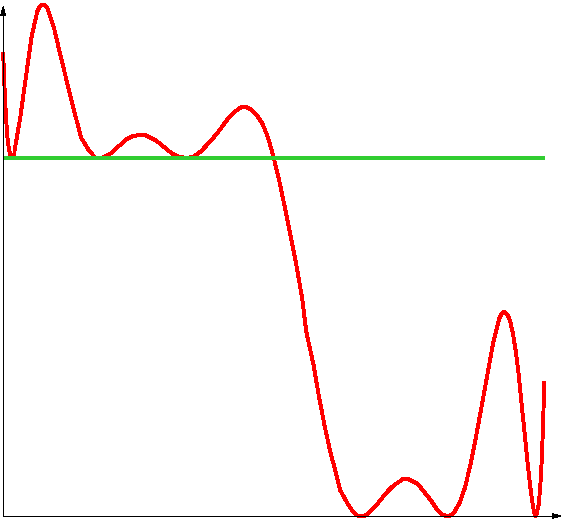
\includegraphics{Estieltjes_1.pdf}
   \caption{Graphe de $T$ pour $n=7$ et $k=4$}
   \label{fig:Estieltjes_1}
\end{figure}

\subsection*{Partie II}
Pour chaque entier $i$ entre $1$ et $n$ et différent de $k$, on définit un polynôme $\Lambda_i$  par :
\begin{displaymath}
\Lambda_i = (X-x_i)(X-x_k)\prod_{j\in\{1,\cdots,n\}-\{i,k\}}(X-x_j)^2
\end{displaymath}
\begin{enumerate}
\item Préciser pour tout couple $(i,j)$ d'entiers entre 1 et $n$ les valeurs de $\widetilde{L_i}(x_j)$.
\item Montrer que $(L_1,\cdots,L_n)$ est une base de $A$. Préciser les coordonnées d'un polynôme $P$ dans cette base.
\item Pour tout $i$ différent de $k$ entre $1$ et $n$, montrer que $\widetilde{\Lambda'_i}(x_i) \neq 0 $ et que
\begin{align*}
 \forall j\in \{1,\cdots ,n\} : \widetilde{\Lambda_i}(x_j)&=0 \\
 \forall j\in \{1,\cdots ,n\} \text{ tel que } j\neq i \text{ et } j\neq k: \widetilde{\Lambda'_i}(x_j)&=0
\end{align*}
\item \begin{enumerate}
\item Montrer que 
\begin{displaymath}
 \left( L_1,\cdots,L_n,\Lambda_1,\cdots,\Lambda_{k-1},\Lambda_{k+1},\cdots,\Lambda_n\right) 
\end{displaymath}
est une base de $E$.
\item Calculer les coordonnées de $T$ dans cette base.
\end{enumerate}
\item \begin{enumerate}
\item Montrer que $T'$ admet $2n-3$ racines distinctes et préciser leurs positions par rapport aux $x_i$.
\item {\'E}tudier les variations de $T$.
\item Montrer que :
\begin{align*}
\forall t \leq x_1 &: \widetilde{T}(t)\geq 1\\
\forall t \in \R &: \widetilde{T}(t)\geq 0 
\end{align*}
Que peut-on conclure pour le coefficient dominant de $T$ ?
\end{enumerate}
\end{enumerate} 
